\let\negmedspace\undefined
\let\negthickspace\undefined
\documentclass[journal,12pt,onecolumn]{IEEEtran}
\usepackage{cite}
\usepackage{amsmath,amssymb,amsfonts,amsthm}
\usepackage{algorithmic}
\usepackage{graphicx}
\usepackage{textcomp}
\usepackage{xcolor}
\usepackage{txfonts}
\usepackage{listings}
\usepackage{enumitem}
\usepackage{mathtools}
\usepackage{gensymb}
\usepackage{comment}
\usepackage{caption}
\usepackage[breaklinks=true]{hyperref}
\usepackage{tkz-euclide} 
\usepackage{listings}

\usepackage{gvv}                                        
%\def\inputGnumericTable{}                                 
\usepackage[latin1]{inputenc}     
\usepackage{xparse}
\usepackage{color}                                            
\usepackage{array}                                            
\usepackage{longtable}                                       
\usepackage{calc}                                             
\usepackage{multirow}
\usepackage{multicol}
\usepackage{hhline}                                           
\usepackage{ifthen}                                           
\usepackage{lscape}
\usepackage{tabularx}
\usepackage{array}
\usepackage{float}
%\newtheorem{theorem}{Theorem}[section]
%\newtheorem{theorem}{Theorem}[section]
%\newtheorem{problem}{Problem}
%\newtheorem{proposition}{Proposition}[section]
%\newtheorem{lemma}{Lemma}[section]
%\newtheorem{corollary}[theorem]{Corollary}
%\newtheorem{example}{Example}[section]
%\newtheorem{definition}[problem]{Definition}

\begin{document}

\title{2.7.7}
\author{AI25BTECH11035 - SUJAL RAJANI}
% \maketitle
% \newpage
% \bigskip
%\begin{document}
{\let\newpage\relax\maketitle}
%\renewcommand{\thefigure}{\theenumi}
%\renewcommand{\thetable}{\theenumi}
% \newpage
% \bigskip
\textbf{Question}:
\\
Find the area of the quadrilateral ABCD whose vertices are A(-4,-3), B(3,-1),C(0,5), and D(-4,2).
\\
 \textbf{Solution}
 \\
as given in the question :
\begin{align*}
     \vec{A}=\myvec{-4\\-3\\0},
     \vec{B}=\myvec{3\\-1\\0},
     \vec{C}=\myvec{0\\5\0},
     \vec{D}=\myvec{-4\\-2\\0}
\end{align*}
the position vector joining $\vec{B}$ and $\vec{D}$ =  $\vec{B}$ -  $\vec{D}$ =$\myvec{7\\1\\0}$ 
\\
\\
\\
the position vector joining $\vec{C}$ and $\vec{A}$ =  $\vec{C}$ -  $\vec{A}$ =$\myvec{4\\8\\0}$
\\
\\
\\
\\
the area of quadrilateral ABCD is the vector  product of $\dfrac{1}{2}$ $||($\vec{B}$ -  $\vec{D}$)\times($\vec{C}$ -  $\vec{A}$)||$
\\  
{VECTOR PRODUCT}
\\
let N be a vector :
\begin{align}
    \vec{N}=\myvec{n_1\\n_2\\0}
    \\
    \end{align}
    let M be a vector :
    \begin{align}
    \vec{M}=\myvec{m_1\\m_2\\0}
\end{align}
the vector product of two vectors $\vec{N}$ and $\vec{M}$ is 
\\
\vec{N}X\vec{M} =
\myvec{
n_{23} & m_{23} \\
n_{31} & m_{31} \\
n_{12} & m_{12}
}
=
\myvec{
n_2 m_3 - n_3 m_2 \\
n_3 m_1 - n_1 m_3 \\
n_1 m_2 - n_2 m_1
}
=
\myvec{
1 \times 0 - 0 \times 8 \\
0 \times 7 - 7 \times 0 \\
7 \times 8 - 1 \times 4
}
=
\myvec{
0 \\
0 \\
52
}
\\
\\
area of ABCD is :
\begin{align*}
    \dfrac{1}{2}||(\vec{B}-  \vec{A})X(\vec{C} -  \vec{A})||=\dfrac{1}{2}||\myvec{7\\1\\0}X\myvec{4\\8\\0}||= \dfrac{1}{2}\sqrt{\myvec{0\\0\\52}^T\myvec{0\\0\\52}}=26
    \end{align*}
    \\
    n1=7,n2=1,m1=4,m2=8
        \begin{figure}[H]
    \centering
    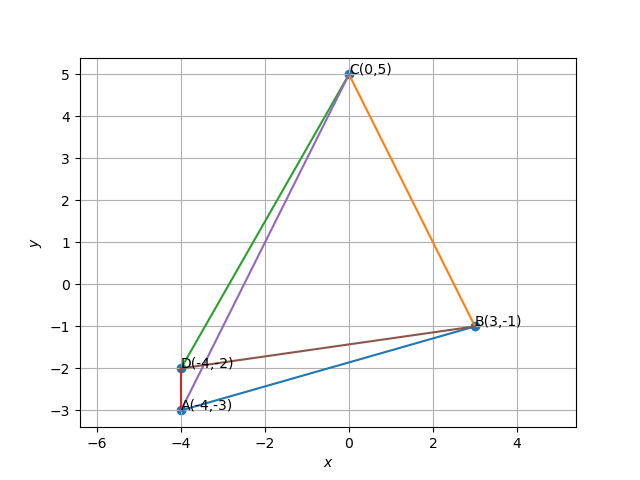
\includegraphics[width = 0.7\columnwidth]{figs/img.png}
    \caption*{}
    \label{figs}
\end{figure}

\end{document}